% !TEX encoding = UTF-8 Unicode.

% Based on https://github.com/Miracle0565/BUCT-Beamer-Theme

\documentclass[
10pt,
aspectratio=43,
]{beamer}
\setbeamercovered{transparent=10}
\usetheme[
%  showheader,
%  red,
  purple,
%  gray,
%  graytitle,
  colorblocks,
%  noframetitlerule,
]{Verona}

\usepackage[T1]{fontenc}
\usepackage{tikz}
\usepackage[utf8]{inputenc}
\usepackage{lipsum}
%%%%%%%%%%%%%%%%%%%%%%%%%%%%%%%
% Mac上使用如下命令声明隶书字体, windows也有相关方式, 大家可自行修改
\providecommand{\lishu}{\CJKfamily{zhli}}
%%%%%%%%%%%%%%%%%%%%%%%%%%%%%%%
\usepackage{tikz}
\usetikzlibrary{fadings}
%
%\setbeamertemplate{sections/subsections in toc}[ball]
\usepackage{xeCJK}
\usepackage{listings}
\usepackage{caption}
\usepackage{subfigure}
\usefonttheme{professionalfonts}
\def\mathfamilydefault{\rmdefault}
\usepackage{amsmath}
\usepackage{multirow}
\usepackage{booktabs}
\usepackage{bm}
\setbeamertemplate{section in toc}{\hspace*{1em}\inserttocsectionnumber.~\inserttocsection\par}
\setbeamertemplate{subsection in toc}{\hspace*{2em}\inserttocsectionnumber.\inserttocsubsectionnumber.~\inserttocsubsection\par}
\setbeamerfont{subsection in toc}{size=\small}
\AtBeginSection[]{%
	\begin{frame}%
		\frametitle{Outline}%
		\textbf{\tableofcontents[currentsection]} %
	\end{frame}%
}

\AtBeginSubsection[]{%
	\begin{frame}%
		\frametitle{Outline}%
		\textbf{\tableofcontents[currentsection, currentsubsection]} %
	\end{frame}%
}

\title{高等数学C}
%\subtitle{A Simple while elegant template}
\author[P.Yu]{余沛}
\mail{peiy\_gzgs@qq.com}
\institute[Guangzhou College of Technology and Business]{Guangzhou College of Technology and Business \\
  广州工商学院}
\date{\today}
\titlegraphic[width=4cm]{logo.png}{}




%%%%%%%%%%%%%%%%%%%%%%%%%%%%%%%%
% ----------- 标题页 ------------
%%%%%%%%%%%%%%%%%%%%%%%%%%%%%%%%



\begin{document}

\maketitle

%%% define code
\defverbatim[colored]\lstI{
	\begin{lstlisting}[language=C++,basicstyle=\ttfamily,keywordstyle=\color{red}]
	int main() {
	// Define variables at the beginning
	// of the block, as in C:
	CStash intStash, stringStash;
	int i;
	char* cp;
	ifstream in;
	string line;
	[...]
	\end{lstlisting}
}
%%%%%%%%%%%%%%%%%%%%%%%%%%%%%%%%
% ----------- FRAME ------------
%%%%%%%%%%%%%%%%%%%%%%%%%%%%%%%%
\section{微分中值定理}

\subsection{Fermat引理}

\begin{frame}{Fermat引理}
	本章将讨论求导这一局部性质的全局效应, 首先给出极值概念.
	\begin{figure}
		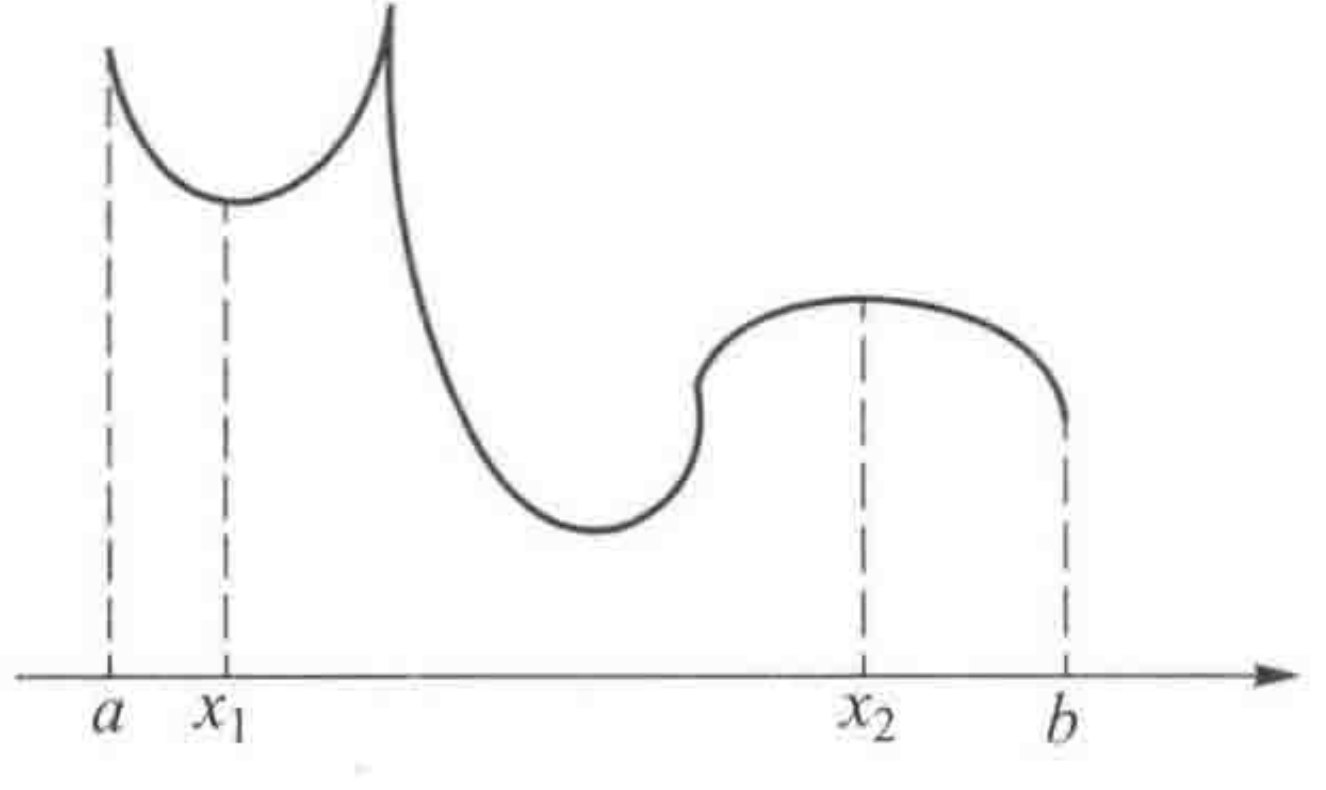
\includegraphics[width=0.45\textwidth]{max-min.png}
	\end{figure}
	\pause
	\begin{block}{定义:极大值与极小值}
		设 $f(x)$ 在 $(a, b)$ 上有定义, $x_0 \in(a$, $b)$, 如果存在点 $x_0$ 的某一个邻域 $O\left(x_0, \delta\right) \subset(a, b)$, 使得
		$$
			f(x) \leqslant f\left(x_0\right), \quad x \in O\left(x_0, \delta\right),
		$$
		则称 $x_0$ 是 $f(x)$ 的一个极大值点, $f\left(x_0\right)$ 称为相应的极大值. 类似地可以定义极小值点和极小值. (在不需要区分极大和极小的时候, 我们将其统称为极值点和极值.)
	\end{block}

\end{frame}

\begin{frame}{Fermat引理}
	在这里, 我们给出第一个临界情况的必要性条件定理, Fermat引理.
	\pause
	\begin{block}{Fermat引理}
		设 $x_0$ 是 $f(x)$ 的一个极值点, 且 $f(x)$ 在 $x_0$ 处导数存在, 则
		$$
			f^{\prime}\left(x_0\right)=0 .
		$$
	\end{block}
	\pause
	\begin{exampleblock}{证明}
		不妨设 $x_0$ 是 $f(x)$ 的极大值点. 由极大值点的定义, 在 $x_0$ 的某个邻域 $O\left(x_0, \delta\right)$上 $f(x)$ 有定义, 且满足
		$$
			f(x) \leqslant f\left(x_0\right),
		$$
	\end{exampleblock}

\end{frame}

\begin{frame}{Fermat引理}
	\begin{exampleblock}{证明}
		于是当 $x<x_0$ 时, 有 $\frac{f(x)-f\left(x_0\right)}{x-x_0} \geqslant 0$; 当 $x>x_0$ 时, 有 $\frac{f(x)-f\left(x_0\right)}{x-x_0} \leqslant 0$. 因为 $f(x)$ 在 $x_0$ 可导, 所以 $f^{\prime}\left(x_0\right)=f_{+}^{\prime}\left(x_0\right)=f_{-}^{\prime}\left(x_0\right)$, 由于
		$$
			f_{-}^{\prime}\left(x_0\right)=\lim _{x \rightarrow x_0^{-}} \frac{f(x)-f\left(x_0\right)}{x-x_0} \geqslant 0, \quad f_{+}^{\prime}\left(x_0\right)=\lim _{x \rightarrow x_0+} \frac{f(x)-f\left(x_0\right)}{x-x_0} \leqslant 0,
		$$
		因此
		$$
			f^{\prime}\left(x_0\right)=0 .
		$$
		同理可证 $x_0$ 为极小值点的情况.
	\end{exampleblock}
	\begin{center}
		\begin{tikzpicture}[scale=0.8]
			% 左边的椭圆框
			\draw[thick] (-3,0) ellipse (2.125cm and 1.275cm);
			\node at (-3,0) {求极值};
			\pause
			% 箭头连接
			\draw[->, thick] (-0.7,0) -- (0.7,0);
			\pause
			% 右边的椭圆框
			\draw[thick] (3,0) ellipse (2.125cm and 1.275cm);
			\node at (3,0) {Euler-Lagrange方程};

		\end{tikzpicture}
	\end{center}

\end{frame}



\subsection{Rolle定理}
\begin{frame}{Rolle定理}
	\begin{block}{Rolle定理}
		设函数$f(x)$满足以下条件:
		\begin{enumerate}
			\item $f(x)$在闭区间$[a, b]$上连续.
			\item $f(x)$在开区间$(a, b)$上可导.
			\item $f(a) = f(b)$.
		\end{enumerate}
		那么在开区间$(a, b)$内至少存在一个数$c$, 使得$f'(c) = 0$.
	\end{block}

	\pause

	\begin{example}
		考虑函数$f(x) = x^2 - 4x + 3$在区间$[1, 3]$上的情况. 我们可以看到$f(x)$满足Rolle定理的所有条件. 因此, 在区间$(1, 3)$内至少存在一个数$c$, 使得$f'(c) = 0$.
	\end{example}
\end{frame}


\begin{frame}{Rolle定理的证明}
	\begin{proof}
		由闭区间上连续函数的性质, 存在 $\xi, \eta \in[a, b]$, 满足
		$$
			f(\xi)=M \quad \text { 和 } f(\eta)=m,
		$$

		其中 $M$ 和 $m$ 分别是 $f(x)$ 在 $[a, b]$ 上的最大值和最小值. 现分两种情况:
		\begin{enumerate}
			\item $M=m$. 此时 $f(x)$ 在 $[a, b]$ 上恒为常数, 结论显然成立.
			\item $M>m$. 这时 $M$ 和 $m$ 中至少有一个与 $f(a)$ (亦即 $f(b))$ 不相同, 不妨设 $M=f(\xi)>f(a)=f(b)$,

			      因此 $\xi \in(a, b)$ 显然是极大值点, 由 Fermat 引理
			      $$
				      f^{\prime}(\xi)=0 .
			      $$
		\end{enumerate}
	\end{proof}
\end{frame}

\subsection{Lagrange定理}

\begin{frame}{Rolle定理, 但 $f(a)\neq f(b)$}
	\begin{columns}[T]
		\begin{column}{0.55\textwidth}
			\begin{itemize}
				\item $f(a)=f(b)$只表示曲线$y=f(x)$在$[a, b]$上的端点$(a, f(a))$和$(b, f(b))$与$x$轴的距离相等. \pause
				\item 若$f(a) \neq f(b)$, 我们保持原点不动, 适当旋转坐标轴, 建立新的坐标系$Ox^{\prime}y^{\prime}$, 使$x^{\prime}$轴平行于$(a, f(a))$和$(b, f(b))$的连线. \pause
				\item 在新的坐标系下, 这段曲线就满足Rolle定理的全部条件. 因此, 存在着曲线上一点, 使曲线在该点处的切线平行于$x^{\prime}$轴, 即与$(a, f(a))$和$(b, f(b))$的连线平行. \pause
			\end{itemize}
		\end{column}
		\begin{column}{0.4\textwidth}
			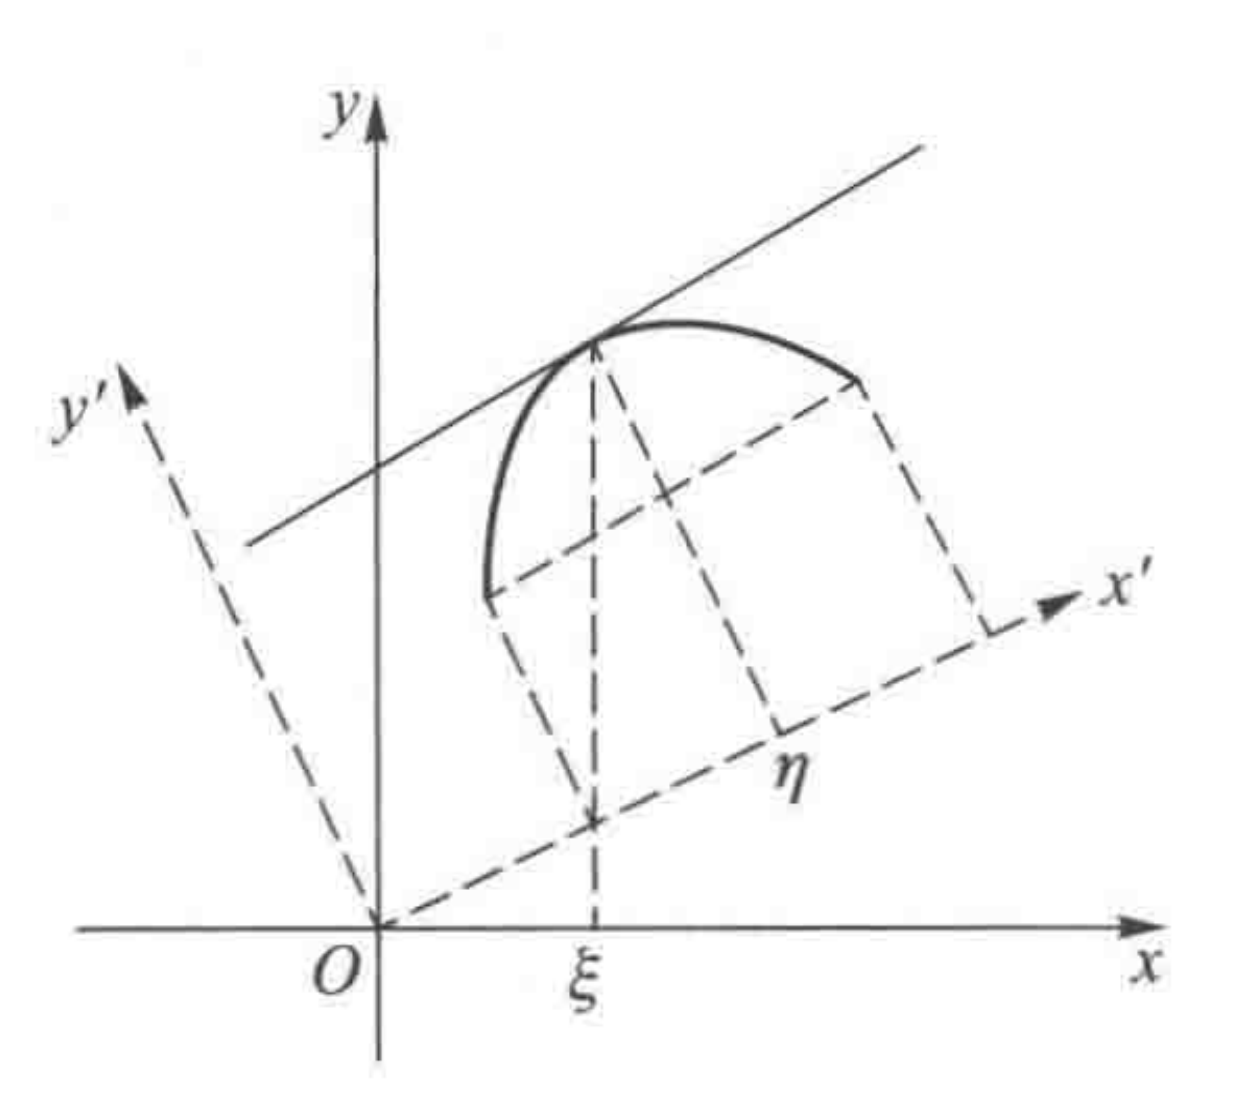
\includegraphics[width=\textwidth]{rolle-lagrange.png}
		\end{column}
	\end{columns}
	\vspace{0.5cm}
	\begin{itemize}
		\item 设该切点在原坐标系中的横坐标为 $x=\xi$, 则切线的斜率 $f^{\prime}(\xi)$ 与 $(a, f(a))$ 和 $(b$, $f(b))$ 的连线的斜率
		      $$
			      \tan \theta=\frac{f(b)-f(a)}{b-a}.
		      $$
	\end{itemize}
\end{frame}

\begin{frame}{Lagrange定理}
	\begin{block}{定理陈述}
		设函数$f(x)$满足以下条件:
		\begin{enumerate}
			\item $f(x)$在闭区间$[a, b]$上连续.
			\item $f(x)$在开区间$(a, b)$上可导.
		\end{enumerate}
		那么在开区间$(a, b)$内至少存在一个数$c$, 使得$f(b) - f(a) = f'(c)(b - a)$.
	\end{block}

	\pause

	\begin{example}
		考虑函数$f(x) = x^2$在区间$[1, 3]$上的情况. 我们可以看到$f(x)$满足Lagrange定理的所有条件. 因此, 在区间$(1, 3)$内至少存在一个数$c$, 使得$f(3) - f(1) = f'(c)(3 - 1)$.
	\end{example}
\end{frame}

\begin{frame}[t]{Lagrange中值定理的证明} \begin{columns}[onlytextwidth] \begin{column}{0.6\textwidth} \begin{proof} 证 作辅助函数
				$$ \varphi(x)=f(x)-f(a)-\frac{f(b)-f(a)}{b-a}(x-a), $$

				由于函数 $f(x)$ 的性质, 函数 $\varphi(x)$ 也在闭区间 $[a, b]$ 上连续,在开区间 $(a, b)$ 上可导,并且有
				$$
					\varphi(a)=\varphi(b)=0,
				$$

				于是由 Rolle 定理, 至少存在一点 $\xi \in(a, b)$, 使得 $\varphi^{\prime}(\xi)=0$. 整理后便得到
				$$
					f^{\prime}(\xi)=\frac{f(b)-f(a)}{b-a} .
				$$
			\end{proof}
		\end{column}
		\begin{column}{0.4\textwidth}
			\begin{figure}
				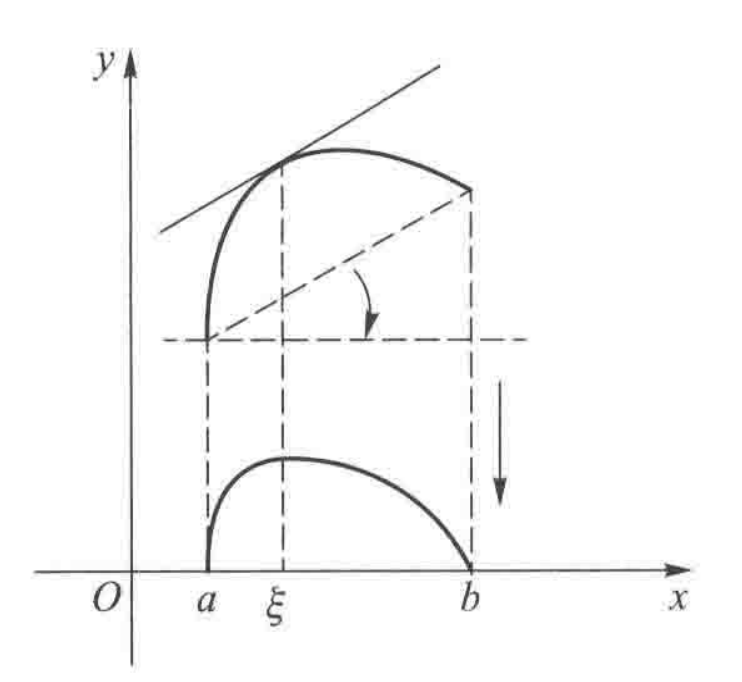
\includegraphics[width=0.88\linewidth]{phi-function.png}
			\end{figure}
		\end{column}
	\end{columns}
\end{frame}

\begin{frame}{Lagrange 中值定理的应用}
	\begin{theorem}[常数函数的判定]
		若 $f(x)$ 在 $(a, b)$ 上可导且有 $f^{\prime}(x) \equiv 0$, 则 $f(x)$ 在 $(a, b)$ 上恒为常数.
	\end{theorem}
	\begin{theorem}[一阶导数与单调性的关系]
		设函数 $f(x)$ 在区间 $I$ 上可导, 则 $f(x)$ 在 $I$ 上单调增加的充分必要条件是: 对于任意 $x \in I$ 有 $f^{\prime}(x) \geqslant 0$;特别地, 若对于任意 $x \in I$ 有 $f^{\prime}(x)>0$, 则 $f(x)$ 在 $I$ 上严格单调增加.
	\end{theorem}
	Why? 试着从函数单调性定义进行分析.
\end{frame}

\begin{frame}{Lagrange 中值定理的应用}
	\begin{block}{定义: 下凸与严格下凸}
		设函数 $f(x)$ 在区间 $I$ 上定义, 若对 $I$ 中的任意两点 $x_1$ 和 $x_2$, 和任意 $\lambda \in(0,1)$, 都有
		$$
			f\left(\lambda x_1+(1-\lambda) x_2\right) \leqslant \lambda f\left(x_1\right)+(1-\lambda) f\left(x_2\right) \text {, }
		$$
		则称 $f(x)$ 是 $I$ 上的下凸函数.
		若不等号严格成立, 则称 $f(x)$ 在 $I$ 上是严格下凸函数.
	\end{block}
	\begin{theorem}[二阶导数与凸性的关系]
		设函数 $f(x)$ 在区间 $I$ 上二阶可导,则 $f(x)$在区间 $I$ 上是下凸函数的充分必要条件是: 对于任意 $x \in I$ 有 $f^{\prime \prime}(x) \geqslant 0$.
	\end{theorem}
\end{frame}

\subsection{Cauchy中值定理}
\begin{frame}{Cauchy中值定理}
	\begin{block}{定理陈述}
		设函数$f(x)$和$g(x)$满足以下条件:
		\begin{enumerate}
			\item $f(x)$和$g(x)$在闭区间$[a, b]$上连续.
			\item $f(x)$和$g(x)$在开区间$(a, b)$上可导.
			\item $g'(x) \neq 0$, 即$g(x)$在$(a, b)$上不恒为零.
		\end{enumerate}
		则至少存在一点 $\xi \in(a, b)$, 使得
		$$
			\frac{f^{\prime}(\xi)}{g^{\prime}(\xi)}=\frac{f(b)-f(a)}{g(b)-g(a)} .
		$$
	\end{block}

	\pause

	\begin{example}
		考虑函数$f(x) = \sin(x)$和$g(x) = \cos(x)$. 可以看到在区间$(0, \frac{\pi}{2})$内至少存在一个数$c$, 使得
		$$
			\frac{\cos(c)}{-\sin(c)}=\frac{\sin(\frac{\pi}{2}) - \sin(0)}{\cos(\frac{\pi}{2}) - \cos(0)}.
		$$
	\end{example}
\end{frame}

\begin{frame}{Cauchy中值定理的证明}
	\begin{block}{Proof.}
		不妨设 $g(x)$ 严格单调增加.	记 $g(a)=\alpha, g(b)=\beta$, 那么 在 $[\alpha, \beta]$ 上存在 $g(x)$ 的反函数 $g^{-1}(y), g^{-1}(y)$, 而且该反函数在 $[\alpha, \beta]$ 上连续, 在 $(\alpha, \beta)$ 上可导, 其导数
		$$
			\left[g^{-1}(y)\right]^{\prime}=\frac{1}{g^{\prime}(x)},
		$$

		并且 $g^{-1}(y)$ 在 $[\alpha, \beta]$ 上也是严格单调增加的. \pause
		考虑 $[\alpha, \beta]$ 上的复合函数 $F(y)=f\left(g^{-1}(y)\right)$, 有 $F(y)$在 $[\alpha, \beta]$ 上满足 Lagrange 中值定理的条件. \pause 于是, 存在 $\eta \in(\alpha, \beta)$, 使得
		$$
			F^{\prime}(\eta)=\frac{F(\beta)-F(\alpha)}{\beta-\alpha}=\frac{f\left(g^{-1}(\beta)\right)-f\left(g^{-1}(\alpha)\right)}{\beta-\alpha}=\frac{f(b)-f(a)}{g(b)-g(a)} .
		$$

	\end{block}
\end{frame}


\begin{frame}{Cauchy中值定理的证明}
	\begin{proof}
		由 $g(x)$ 和 $g^{-1}(y)$ 的关系, 在 $(a, b)$ 中一定存在一点 $\xi$, 满足 $g(\xi)=\eta$, 于是
		$$
			\begin{aligned}
				F^{\prime}(\eta) & =\left.\left\{f\left(g^{-1}(y)\right)\right\}^{\prime}\right|_{y=\eta}                                                                  \\
				                 & =\left.\left\{f^{\prime}\left(g^{-1}(y)\right) \cdot\left[g^{-1}(y)\right]^{\prime}\right\}\right|_{y=\eta}                             \\
				                 & =\left.\left\{f^{\prime}(x) \cdot \frac{1}{g^{\prime}(x)}\right\}\right|_{x=g^{-1}(\eta)=\xi}=\frac{f^{\prime}(\xi)}{g^{\prime}(\xi)} .
			\end{aligned}
		$$
	\end{proof}
\end{frame}

\section{L'Hôpital 法则 (洛必达法则)}
\subsection{{L'Hôpital法则 (洛必达法则)}的证明}
\begin{frame}{L'Hôpital法则 (洛必达法则)}
	\begin{theorem}[L'Hôpital法则]
		设函数 $f(x)$ 和 $g(x)$ 在 $(a, a+d]$ 上可导 $(d$ 是某个正常数), 且 $g^{\prime}(x) \neq 0$. 若此时有
		$$
			\lim _{x \rightarrow a+} f(x)=\lim _{x \rightarrow a^{+}} g(x)=0
		$$

		或
		$$
			\lim _{x \rightarrow a^{+}} g(x)=\infty,
		$$

		且 $\displaystyle\lim _{x \rightarrow a+} \frac{f^{\prime}(x)}{g^{\prime}(x)}$ 存在$($可以是有限数或 $\infty)$, 则
		$$
			\lim _{x \rightarrow a^{+}} \frac{f(x)}{g(x)}=\lim _{x \rightarrow a^{+}} \frac{f^{\prime}(x)}{g^{\prime}(x)} .
		$$
		同理, 对$x\to a^-,\,\,x\to a,\,\,x\to\infty,\,\,x\to -\infty$ 有类似结果.
	\end{theorem}

\end{frame}

\begin{frame}{L'Hôpital法则 (洛必达法则)}
	\begin{exampleblock}{证明概要}
		\begin{itemize}
			\item $\displaystyle\lim _{x \rightarrow a^{+}} f(x)=\lim _{x \rightarrow a^{+}} g(x)=0$ 的情形: 补充定义 $f(a)=g(a)=0$, 可以有
			      $$
				      \frac{f(x)}{g(x)}=\frac{f(x)-f(a)}{g(x)-g(a)}=\frac{f^{\prime}(\xi)}{g^{\prime}(\xi)} .
			      $$
			\item $\displaystyle\lim _{x \rightarrow a^{+}} g(x)=\infty$ 的情形:
			      $$
				      \begin{aligned}
					      \frac{f(x)}{g(x)} & =\frac{f(x)-f\left(x_0\right)}{g(x)}+\frac{f\left(x_0\right)}{g(x)}                                                                   \\
					                        & =\frac{g(x)-g\left(x_0\right)}{g(x)} \cdot \frac{f(x)-f\left(x_0\right)}{g(x)-g\left(x_0\right)}+\frac{f\left(x_0\right)}{g(x)}       \\
					                        & =\left[1-\frac{g\left(x_0\right)}{g(x)}\right] \frac{f(x)-f\left(x_0\right)}{g(x)-g\left(x_0\right)}+\frac{f\left(x_0\right)}{g(x)} .
				      \end{aligned}
			      $$
		\end{itemize}
	\end{exampleblock}
\end{frame}

\begin{frame}[fragile]{求极限}
	\begin{block}{问题}
		\begin{columns}[onlytextwidth]
			\column{0.5\textwidth}
			\begin{enumerate}
				\item $\displaystyle\lim _{x \rightarrow 0} \frac{e^x-e^{-x}}{\sin x}$;
				\item $\displaystyle\lim _{x \rightarrow \pi } \frac{\sin 3 x}{\tan 5 x}$;
				\item $\displaystyle\lim _{x \rightarrow \frac{\pi}{2}} \frac{\ln (\sin x)}{(\pi-2 x)^2}$;
			\end{enumerate}
			\column{0.5\textwidth}
			\begin{enumerate} \setcounter{enumi}{3}
				\item $\displaystyle\lim _{x \rightarrow a} \frac{x^m-a^m}{x^n-a^n}$;
				\item $\displaystyle\lim _{x \rightarrow 0+} \frac{\ln (\tan 7 x)}{\ln (\tan 2 x)}$;
				\item $\displaystyle\lim _{x \rightarrow \frac{\pi}{2}} \frac{\tan 3 x}{\tan x}$.
			\end{enumerate}
		\end{columns}
	\end{block}

	\pause

	\begin{exampleblock}{答案}
		\begin{columns}[onlytextwidth]
			\column{0.5\textwidth}
			\begin{enumerate}
				\item $\displaystyle\lim _{x \rightarrow 0} \frac{e^x-e^{-x}}{\sin x} = 2$; \pause
				\item $\displaystyle\lim _{x \rightarrow \pi } \frac{\sin 3 x}{\tan 5 x} = \frac{3}{5}$; \pause
				\item $\displaystyle\lim _{x \rightarrow \frac{\pi}{2}} \frac{\ln (\sin x)}{(\pi-2 x)^2} = \frac{-1}{\pi^2}$; \pause
			\end{enumerate}
			\column{0.5\textwidth}
			\begin{enumerate} \setcounter{enumi}{3}
				\item $\displaystyle\lim _{x \rightarrow a} \frac{x^m-a^m}{x^n-a^n} = \frac{m a^{m-1}}{n a^{n-1}}$; \pause
				\item $\displaystyle\lim _{x \rightarrow 0+} \frac{\ln (\tan 7 x)}{\ln (\tan 2 x)} = 1$; \pause
				\item $\displaystyle\lim _{x \rightarrow \frac{\pi}{2}} \frac{\tan 3 x}{\tan x} = 3.$
			\end{enumerate}
		\end{columns}
	\end{exampleblock}
\end{frame}

\subsection{更进一步的求极限方法}
\begin{frame} \frametitle{欲求的极限和变换方法}

	\everymath{\displaystyle}

	\begin{block}{$0\cdot\infty$型} 
		若 $\lim _{x \rightarrow c} f(x)=0, \lim _{x \rightarrow c} g(x)=\infty$, \\
		可计算
		$$\lim _{x \rightarrow c} f(x) g(x)=\lim _{x \rightarrow c} \frac{f(x)}{1 / g(x)}$$ 或 $$\lim _{x \rightarrow c} \frac{g(x)}{1 / f(x)}$$
	\end{block}
\pause
	\begin{block}{$\infty-\infty$ 型}
		若$\lim _{x \rightarrow c} f(x)=\infty, \lim _{x \rightarrow c} g(x)=\infty$, \\
		可计算$$\lim _{x \rightarrow c}(f(x)-g(x))=\lim _{x \rightarrow c} \frac{1 / g(x)-1 / f(x)}{1 /(f(x) g(x))}.$$
	\end{block}

\end{frame}

\begin{frame} \frametitle{欲求的极限和变换方法}

	\everymath{\displaystyle}

	\begin{block}{$(0^+)^0$ 型与$\infty^0$ 型} 
		若$\lim _{x \rightarrow c} f(x)=0^{+}, \lim _{x \rightarrow c} g(x)=0$ 或 $\lim _{x \rightarrow c} f(x)=\infty, \lim _{x \rightarrow c} g(x)=0$, \\
		可计算$$\lim _{x \rightarrow c} f(x)^{g(x)}=\exp \lim _{x \rightarrow c} \frac{g(x)}{1 / \ln f(x)}.$$
	\end{block}
\pause
	\begin{block}{$1^\infty$ 型} 
		若$\lim _{x \rightarrow c} f(x)=1, \lim _{x \rightarrow c} g(x)=\infty$, 可计算 \\
		$$\lim _{x \rightarrow c} f(x)^{g(x)}=\exp \lim _{x \rightarrow c} \frac{\ln f(x)}{1 / g(x)}.$$
	\end{block}

\end{frame}


% Thank you page
\beamertemplateshadingbackground{structure.fg!90}{structure.fg}
\begin{frame}[plain]
	\vfill
	\centering
	{
	\centering \Huge \color{white} Thank you for your attention!\\[10pt]Questions?\\ [10pt] Homework: Page167: 1, 2, 3, 9, Page168: 10.
	}
	\vfill
\end{frame}


\end{document}


